\documentclass{article}
\usepackage[left=0.5in,top=0.5in,right=0.5in,bottom=0.5in]{geometry}
\usepackage[dvipsnames]{xcolor}
\usepackage[english]{babel}
\usepackage[utf8]{inputenc}
\usepackage{graphicx}
\usepackage{
  amssymb,
  amsmath,
  amsthm,
  latexsym
}
\graphicspath{{./images/}}
\title{Moth Evolution Simulation Lab Report}
\author{Philip Kim}
\date{\today}
\begin{document}
\maketitle
\begin{enumerate}
  \item After the conclusion of this simulation, log your results. Start this by attaching a screenshot of your graph. In which direction did the allele frequencies change?
  \begin{center}
    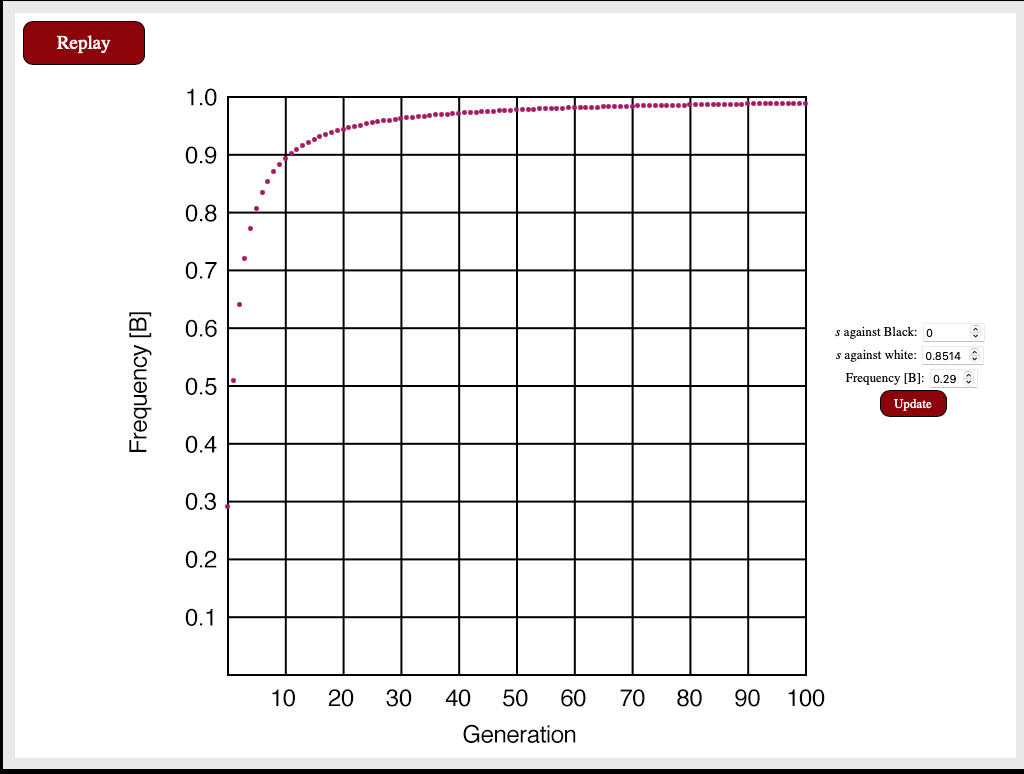
\includegraphics[scale=0.3]{white.png}
  \end{center}
  \begin{itemize}
    \item The frequency of the black allele in the population after 100 generations increased up to almost 1.
  \end{itemize}
  \item Explain the mechanism by which these changes occurred. What is this mechanism called?
  \begin{itemize}
    \item Microevolution is caused only by five processes: selection, mutation, non-random mating, genetic drift, and isolation.
  \end{itemize}
  \item Which of the three genotypes do you think would be most fit in a rural area, far from cities, such as the woods in the far South of England?
  \begin{itemize}
    \item
  \end{itemize}
  \item Which of the three genotypes do you think would be most fit in the woods near industrial cities?
  \begin{itemize}
    \item
  \end{itemize}
  \item What do you think happened after England passed clean air laws?
  \begin{itemize}
    \item
  \end{itemize}
  \item Play around with the simulation and change the ``selection against Black, selection against White.'' What do you notice?
  \begin{itemize}
    \item It has an inverse relationship.
  \end{itemize}
\end{enumerate}
\end{document}